\chapter{The Fundamentals}

  The purpose of this document is to provide an overview of the MeqTree kernel
  and related interfaces. The following subjects will be covered:

  \begin{itemize}

  \item Basic terms and concepts.

  \item System components.

  \item Data structures employed in the MeqTree kernel.

  \item Standard node state \& functionality.

  \item Interaction between nodes, and how it is affected by state.

  \item Interaction with Glish (and in the future, other scripting languages).

  \item Examples of some standard and application-specific nodes.

  \end{itemize}

  The intended audience for this document is:

  \begin{description}

  \item[The Tree Designer,] since a thorough understanding of how nodes interact
  is critical in construction of complex and efficient trees.

  \item[The Node Developer] needing to implement specialized node classes.

  \end{description}


\section{Trees}

  The MeqTree kernel provides a C++ implementation of the MeqTree concept. A {\bf
  MeqTree} (or simply ``tree'') is a collection of interconnected {\bf MeqNodes}
  (or simply ``nodes''). Nodes have a directed parent--child relationship; a
  parent may have any number of children, and a child can have multiple parents.
  Cycles are forbidden. Technically, this makes the MeqTree a {\em directed
  acyclic graph}, but the term ``tree'' is retained for historical and
  aesthetical reasons.

  We will often use directional terms when discussing trees, {\bf up} is from
  parent to child, and {\bf down} is from child to parent.

  In broad terms, the life of a node generally consists of receiving {\bf
  requests} from its parent(s), passing them on to its children, receiving {\bf
  results} in response, performing some calculation on the child results, and
  returning the result of that its parent. Thus, requests generally originate
  somewhere down the tree and propagate up, while results germinate at the top
  and percolate down. 

\section{The math}
  \label{sec:math}

  \newcommand{\RR}{\mathcal{R}}
  \newcommand{\CC}{\mathcal{C}}
  \newcommand{\PP}{\mathcal{P}}

  Trees are mostly concerned with evaluating functions (e.g., predicted
  visibilities), optionally comparing these functions to other functions (e.g.,
  measured visibilities), and solving for adjustable parameters to obtain the
  best fit. Before we discuss this in detail, it helps to define some basic 
  mathematical terms.

  The result of a node usually represents some function defined over
  $\mathcal{R}^2$ space -- $f:\RR^2\rightarrow\RR^N$ or
  $f:\RR^2\rightarrow\CC^N$. The $\mathcal{R}^2$ domain is interpreted as
  frequency--time space in our application context, but in fact there's very
  few places in the kernel where this has any specific meaning. The codomain,
  $\RR^N$ or $\CC^N$, could represent any number of things, e.g., a single
  visbility $XX\subset\CC$, the Stokes parameters $(IQUV)\subset\RR^4$, four
  complex visibilities in $\CC^4$, etc.

  The actual function {\bf domain} $[x_1,x_2]\times[y_1,y_2]$  is a rectangular
  subset of $\RR^2$. Within the domain, we work with sets of $N\times M$ {\bf
  cells}. Each cell ${\mathbf c}_{ij}$ is a $\Delta x_i\times\Delta y_j$
  rectangle, centered on point $(x_i,y_j)$. The function itself is represented
  by an object called the {\bf vells}, which is essentially a set of $N\times
  M$ {\em samplings}\/ $\{f_{ij}\}$:  $$f_{ij}=f(x_i,y_j),$$ or $N\times M$
  {\em integrations}\/ $\{\tilde{f}_{ij}\}$: $$
  \tilde{f}_{ij}=\mathop{\int\!\!\!\int}_{{\mathbf c}_{ij}}f(x,y)\,dx\,dy.$$
  
  A vells $\{f_{ij}\}$ can also represent a set of {\em measured data}, such as
  observed complex visibilities. 
  
  A function may also depend on $K$ real parameters. If we designate the {\em
  parameter space} $\PP:=\RR^K$, then our function essentially becomes
  $f:\RR^2\times\PP\rightarrow\RR^N$ or $f:\RR^2\times\PP\rightarrow\CC^N$.
  This can also be represented as $f(x,y;p_1...p_K)$, or $f(x,y;\vec{p})$. The
  {\em model fitting problem} is essentially a minimization problem: finding
  the value $\vec{p}_0$  that minimizes the function $\chi^2(x,y;\vec{p})$ over
  a fixed set of cells in $(x,y)$ space. The $\chi^2$ function  ties together
  {\em predicted data} $f(x,y;\vec{p})$, measured data $\{\hat{f}_{ij}\}$, and
  an optional set of weights $\{w_{ij}\}$:

  $$ \chi^2(\vec{p}) = \sum_{ij} (f(x_i,y_j;\vec{p}) - \hat{f}_{ij})^2w_{ij},$$
  
  Solving the minimization problem hinges on estimating the gradients of $f$ in
  $\PP$ space.\footnote{The expressions are slightly different when dealing
  with integrations (as we do in the case of visibilities), but the operational
  principle remains the same.} Given a tree that computes $f_{ij}=f(x_i,y_j;\vec{p})$, we can
  numerically estimate each partial derivative ${\partial f}/{\partial
  p_k}(x,y;\vec{p})$ by taking a small {\bf perturbation} $\delta_k$, and using
  the same tree to compute the {\bf perturbed values} $f^{(k)}_{ij} =
  f(x_i,y_j;p_1,...,p_{k-1},p_k+\delta_k,p_{k+1},...,p_{K})$. In fact, trees are
  designed to automatically compute perturbed values along with the function
  value. These are returned as a {\bf vellset}, which is composed of the {\em
  value vells} $\{f_{ij}\}$, and $K$ {\em perturbed value vells}
  $\{f^{(k)}_{ij}\}$.
  

\section{Nodes}

  Nodes are implemented as C++ objects, subclassed from the abstract
  \qq{Meq::Node} class\footnote{All the MeqTree kernel classes reside in the
  \qq{Meq} namespace; we will omit \qq{Meq::} from names from now on.}. All
  interaction with nodes is done via the \Node\ class interface. Consequently, a
  node has no direct knowledge of the {\em type} of its children. Nodes may be
  connected together in a practically arbitrary manner. Given a rich toolbox of
  elementary node classes, trees representing arbitrary mathematical expressions
  may thus be constructed. 

  All nodes have a {\bf state record} that determines their behaviour. The state
  record is fully accessible from the outside. The initial state record is also
  called the {\bf defrec} (from definition record), and is usually supplied from
  the scripting layer when the node is created.

  Nodes also have a {\bf result cache} that may retain the most recently computed
  result. The cache is intended to save processing time for repeated (or similar
  enough) requests.

\section{Design Philosophy}

  These principles are key to understanding the design philosophy behind the
  kernel:

  \begin{description}

  \item[Locality:] all functionality is defined in terms of local parent--child
  request--result interactions. There is no centralized ``control'' as such.

  \item[KISS the nodes and rely on emergent behaviour:] complex behaviour of the
  tree as a whole emerges from primitive request--result interactions at the
  local level. Most node classes are designed to be simple (K.I.S.S.!), with a
  single well-defined purpose. If some sort of specific functionality is
  required, it is almost always preferrable to implement it by building the right
  tree, rather than developing specialized nodes.

  \item[Policy-free:] kernel node classes are largely policy-free. By policy we
  mean any sort of application-specific behaviour or concepts. Policy may only
  emerge at the tree level (by connecting the nodes in a specific way), and/or at
  the scripting level.

  \item[There is more than one way to do it:] (with a nod to Larry Wall and Perl)
  in a lot of cases, the kernel provides several ways of accomplishing the same 
  result. There is not necessarily a single ``right'' way, it all depends on the
  particular application context. This redundancy is by design, as it increases
  the overall adapatability of the system.

  \end{description}

\section{Software components}

  An interface to the kernel is provided via a \qq{MeqServer} object. The
  \qq{MeqServer} maintains a {\bf forest} (a collection of nodes and trees), and
  provides operations such as:

  \begin{itemize}

  \item Create, connect and delete node objects.

  \item Inspect and modify node state records.

  \item Issue requests and return results.

  \item Connect trees to data sources (e.g. Measurement Sets).

  \end{itemize}

  \qq{MeqServer} plugs into the OCTOPUSSY publish/subscribe framework, and
  thorugh it can can transparently support any number of local or remote clients,
  such as Glish sessions.

  All application-dependent logic (``policy'') is meant to reside in the scripting
  layer (Glish, and in the future Python).

\chapter{Data Structures} 

\section{Basic concepts}

  The main priciple driving data structure design in MeqTrees is {\bf
  congruity}: all C++ objects used to {\em pass information} within a tree must
  be mappable without any loss of information to and from data structures on
  the scripting side. Fully {\em private} structures (e.g., private nested
  classes) can exist on the C++ side only.

  Congruity facilitates {\bf transparency}: most of the inner workings of a
  tree are readily accessible from the scripting side. This allows for very
  elaborate monitoring schemes, and is a great debugging aid when something
  goes wrong.

\subsection{Data types}
  
  The choice of atomic data types is limited by the requirement of congruity.
  Currently, the only supported scripting language is Glish, but Python 
  support is expected in the near future. In any case, the kernel  restricts
  itself to common primitives that are supported by all mature scripting
  languages. Thus, kernel data structures are defined in terms of a restricted
  set of ``legal data objects'', specifically:

  \begin{itemize}
  
  \item scalars -- bool, integer, float, double, float or double complex;
  
  \item strings;
  
  \item multidimensional arrays of scalars;
  
  \item lists of legal objects (in Glish this is represented either  via a
  vector of scalars or strings, or via a record with fields indexed by number);

  \item records of legal objects (a.k.a. dictionaries/maps/hashes with a string
  key and a legal object value).

  \end{itemize}

  On the C++ side, data objects are based on the DMI \qq{DataRecord},
  \qq{DataField} and \qq{DataArray} classes. Most data classes are in fact
  derived from \qq{DataRecord}, and are at core a record with some (sometimes
  loosely) predefined structure.

\subsection{HIIDs}

  The \qq{HIID} (hierarchical indentifier) class of the DMI package is used for
  all data-related indentifiers in the kernel, such as record fields, node
  groups, request IDs, etc.
  
  A HIID is essentially a vector of integers called {\em atomic IDs}. Atomic
  IDs have a string representation: for IDs $>=$0 this is simply the integer
  itself in string form, while for IDs $<$0, a global {\em dictionary} (i.e.
  map from strings to numbers) is maintained in the development tree. Another
  way to look at this is that negative IDs represent {\em atomic concepts}, or
  words. Thus, any HIID can be viewed as a mix of words (from a fixed though
  rather large vocabulary!) and numbers.

  The string form of a HIID consists of atomic IDs, separated by periods. For
  example, \qq{"Request.ID.1"} is the string form of $(-1210,-1087,1)$. Note
  that the string form is {\bf not} case-sensitive, so \qq{"request.id.1"}
  corresponds to the same HIID. An alternative string representation, employing
  underscore (\qq{"\_"}) as the separator, is used for Glish record fields,
  e.g., \qq{rec.request\_id\_1}. 

  The reason we use such HIIDs instead of plain strings is efficiency on the
  C++ side -- many data storage classes engage in parsing or building up HIIDs,
  and vectors of integers are much easier to manipulate than strings. Note that
  the symbol-to-ID mapping is also available as C++ header files containing
  \qq{const} declarations for atomic IDs. These may be used as, e.g.:

  \begin{verbatim}
  const HIID MyFieldName = AidRequest | AidId | 1;
  \end{verbatim}
  
  is a convenient and visually obvious way to define a constant HIID
  corresponding to \qq{"Request.ID.1"}. The compiler turns this declaration
  into a constant vector of integers.

  HIIDs are covered in more detail in the documentation for DMI. Here we'll
  only dwell on their Glish form. There's two forms in which HIIDs appear in
  Glish:
  
  \begin{itemize}
  
  \item As record field names, e.g., \qq{rec.request\_id}. The implication of
  this is that in order to be recognized by the kernel, all record field names
  must be built up from a fixed vocabulary (which may be extended by the
  C++ developer as new classes are added).

  \item As values. In Glish, a HIID value is just a string containing the
  HIID's symbolic form, tagged by the \qq{::is\_dmi\_hiid} attribute. The
  \qq{hiid()} function (in \qq{dmitypes.g}) is a convenient way to create HIID
  values. For example:

  \begin{verbatim}
  my_id := hiid('Request.ID.1');
  my_id := hiid('request','id',1);
  \end{verbatim}
  
  will both create the same HIID. 
  
  Note the crucial difference between strings and HIID values. Compare the two
  Glish records:

  \begin{verbatim}
  rec1 := [ a = 'a.b.c.1' ];
  rec2 := [ a = hiid('a.b.c',1) ];
  \end{verbatim}
  
  While they may appear to be practically identical on the Glish side of things
  -- both records contain the string field \qq{a}, except \qq{rec2.a} has an
  extra attribute tag -- when passed to the C++ kernel, \qq{rec1.a} is
  converted to an \qq{std::string} object, while \qq{rec2.a} is converted to a
  \qq{HIID} object.
  
  \end{itemize}

  In this document, we will use both forms interchangably depending on context,
  with the understanding that, e.g., \qq{request\_id\_1} and \qq{"Request.ID.1"}
  both refer to the thing as far as the kernel is concerend.

\subsection{Naming conventions}

  \begin{itemize}

  \item In C++, standard data structures \& nodes reside in \qq{namespace Meq}.
    In Glish, corresponding object constructor functions are placed into the
    {\tt meq} ``namespace'' (actually just a record), and names are
    all-lowercase. The DMI dynamic type system uses a {\tt Meq} prefix for the
    namespace. Thus, the \qq{Meq::\Request} class in C++ is registered as a
    ``\qq{MeqRequest}'' in the DMI type system, and  has a \qq{meq.request()}
    counterpart in Glish.

  \item Even though the languages we use are case-sensitive, HIIDs aren't. A
    good reason to avoid relying character case to distinguish identifiers is
    that different languages and contexts have different capitalization
    conventions -- compare, e.g., \qq{Meq::Request} in C++, as opposed to
    \qq{meq.request} in Glish. Thus we should always avoid assigning
    case-sensitive names to different entities.

  \end{itemize}

\subsection{Glish \qq{meq} objects: meqtypes.g}

  With a couple of exceptions, Meq objects are represented by Glish records of
  a [mostly] predefined layout. The Glish/C++ conversion layer uses a few
  ``magic'' attributes to distinguish these objects from ordinary records, so
  it is able to map them to specialized Meq C++ classes rather than generic
  \qq{DataRecord}s. 

  Specifically, the \qq{::dmi\_actual\_type} attribute is set to a string which
  gives the DMI object type. Thus, it is possible to construct a record in
  Glish, tag it with \qq{::dmi\_actual\_type}, pass it thorugh the Glish/C++
  layer, and have it auto-magically converted to an C++ object of the
  appropriate class. The only requirement is that the record contain the
  correct set of fields, which are mapped to class attributes (data members) in
  C++. The file \qq{meq/meqtypes.g} defines  some Glish ``constructor''
  functions which create properly formed records\footnote{Note that some Meq
  classes may have Glish counterparts but no Glish constructors. At time of
  writing, these include \Vells, \VellSet{}s, and \Result{}s. The reason for
  this is simply lack of necessity, since objects of these classes always
  originate on the C++ side rather than Glish. In the future, constructors for
  these classes may be added to Glish as required.}:

  \begin{description}
  
  \item[\qq{meq.domain()}] creates a Domain object (record).

  \item[\qq{meq.cells()}] creates a Cells object (record).

  \item[\qq{meq.requestid()}] creates a request ID from individual components
  (e.g., domain ID, config ID, iteration ID). A request ID is really just a
  \qq{HIID}.

  \item[\qq{meq.request()}] creates a Request object (record).
  
  \item[\qq{meq.polc()}] creates a Polc object (record).
  
  \end{description}
  
  In general, all data objects on the C++ side have counterparts on the Glish
  side. Within this document, we will usually describe data objects in terms of
  their Glish equivalents -- records and record fields -- with the implied
  understanding that there is a 1:1 mapping from that to C++ classes and data
  members.

\subsection{Glish lists}

  Glish does not have a native ``list'' (a.k.a. ``sequence'') construct.
  Instead, lists are emulated in one of two ways:

  \begin{itemize}

  \item If all list elements are all of the same {\em scalar} type,
  then the list is emulated by a vector.
  
  \item If the list elements are of a non-scalar type, or the type is not
  homogenous, then the list is emulated by a record.\footnote{When mapping lists created
  in the kernel to Glish records, the conversion layer assigns field names of
  the form \qq{"\#1"}, \qq{"\#2"}, etc.}
  \end{itemize}

  Since Glish records support numeric subscripts, both types of lists can be
  accessed via the same syntax -- \qq{len(list)} returns the number of
  elements, \qq{list[$n$]} accesses element $n$. Note though that if a list
  contains only one element, it should still be accessed as \qq{list[1]} rather
  than \qq{list} (the latter syntax will actually do the right thing given a
  vector, but not a record, hence it should be avoided for consistency's sake.)

  We will use the term {\em list} from now on to refer to both types of Glish
  structures, as it should usually be clear from context which type is actually
  employed.


\subsection{1-based and 0-based indexing}
  \label{sec:indexconv}

  Glish array indices are 1-based, while C++ indices are 0-based. This,
  unfortunately, has always lead to all sorts of confusion, since indices pop
  up on both sides of the Glish/C++ barrier, and sometimes even need to be
  passed back and forth. As our experience with AIPS++ has shown, keeping track
  of index conversion on an individual basis is completely impractical.

  {\bf The Glish/C++ conversion layer attempts to address this issue by
  providing {\em automatic conversion} of indices. If a record field's name
  ends in \qq{\_index} (on the C++ side this corresponds to a field HIID ending
  in the atomic ID \qq{"Index"}), and the field contains a single integer or a
  list of integers, then the field is assumed to contain indices, and
  conversion between 0- and 1-base is automatically performed.}

  Thus, the Glish record \qq{[foo=1,foo\_index=1,bar\_index=[2,3]]} will be
  converted to \qq{[Foo=1,Foo.Index=0,Bar.Index=[1,2]]} on the C++ side (and
  vice versa), while \qq{[foo\_index=1.0]} or \qq{[foo\_index=[a=1,b=2]]} will
  not undergo any conversion (since the \qq{\_index} field contains a
  \qq{double} value in one case, and a subrecord in the other case).

  Automatic conversion, of course, introduces its own potential for confusion
  if forgotten about. This is why you simply shouldn't forget about it. As a
  visual aid, the paragraph above is highlighted in bold.

\section{MeqRequest and related data objects}

  A \Request\ is a {\em job description} containing a number of commands that a
  node executes in order to produce a \Result. A \Request\ is implemented as a
  record with a semi-fixed structure; commands correspond to specific field 
  names, while the value of each field usually carries the command arguments.
  
  Operationally, the critically important command is \qq{cells}: this tells the
  node to evaluate itself over a given grid in the frequency--time domain. In
  fact, most other commands are mere housekeeping, while \qq{cells} represents
  the brunt of the workload. For this reason, the \qq{cells} command gets
  special treatment: it is placed at the top level of the request record (along
  with a few related flags), and all nodes are obliged to process it. All other
  commands are kept inside a {\bf rider} sub-record, and are subject to a {\em
  node selection} mechanism that allows commands to be directed to all nodes,
  individual nodes, or groups of nodes (this is described in further detail in
  section~\ref{CSR}).

  Each \Request\ is assigned unique request ID ({\bf rqid}, pronounced
  ``arr-cue-d''). This is a \qq{HIID} describing various properties of the
  request. Request generators are expected to follow a certain {\em contract},
  and assign rqids in a consistent way. This is covered in detail in
  section~\ref{sec:rqid}.

  On the C++ side, a \Request\ is derived from \qq{DataRecord}. It can contain
  the following fields (of which only request\_id is obligatory).
  \vspace{1em}

  \noindent\begin{tabular}{l|l|p{.7\textwidth}}
  \hline
  {\scriptsize\sf field name } & {\scriptsize\sf type} & {\scriptsize\sf description}\\
  \hline
  \qq{request\_id} & \qq{HIID} & the request ID\\
  \qq{cells}       & \qq{Cells} & {\em [optional]}~~a \Cells\ object (see below)\\
  \qq{calc\_deriv} & \qq{int} & {\em [optional]}~~compute perturbed values (0, 1 or 2).
                      Default is 0.\\
  \qq{next\_request} & n/a & {\em [optional]}~~a hint of what the next request is going to be.
                      This influences caching decisions and speculative
                      execution (section~\ref{sec:nextreq}). {\em This is not
                      currently implemented.}\\
  \qq{rider}       & \qq{record} & {\em [optional]}~~rider subrecord containing additional commands.
  \\\hline
  \end{tabular}\vspace{1em}
  
\subsection{Constructing Requests}
  
  In Glish, a \Request\ record can be created by calling the following
  function:

  \begin{verbatim}
  meq.request := function (cells=F,request_id=F,calc_deriv=0)
  \end{verbatim}
  
  You can subsequently add commands to the record using \qq{meq.add\_command()}
  and \qq{meq.add\_state()}. This is also described in section~\ref{sec:CSR}.
  
\subsection{Domains and Cells}

  The \qq{Domain} class represents a rectangular domain in frequency--time
  space. The \qq{Cells} class represents a gridding of that domain. This is
  illustrated by Figure~\ref{fig:cells}.
  
  \begin{figure}
  \begin{centering}
  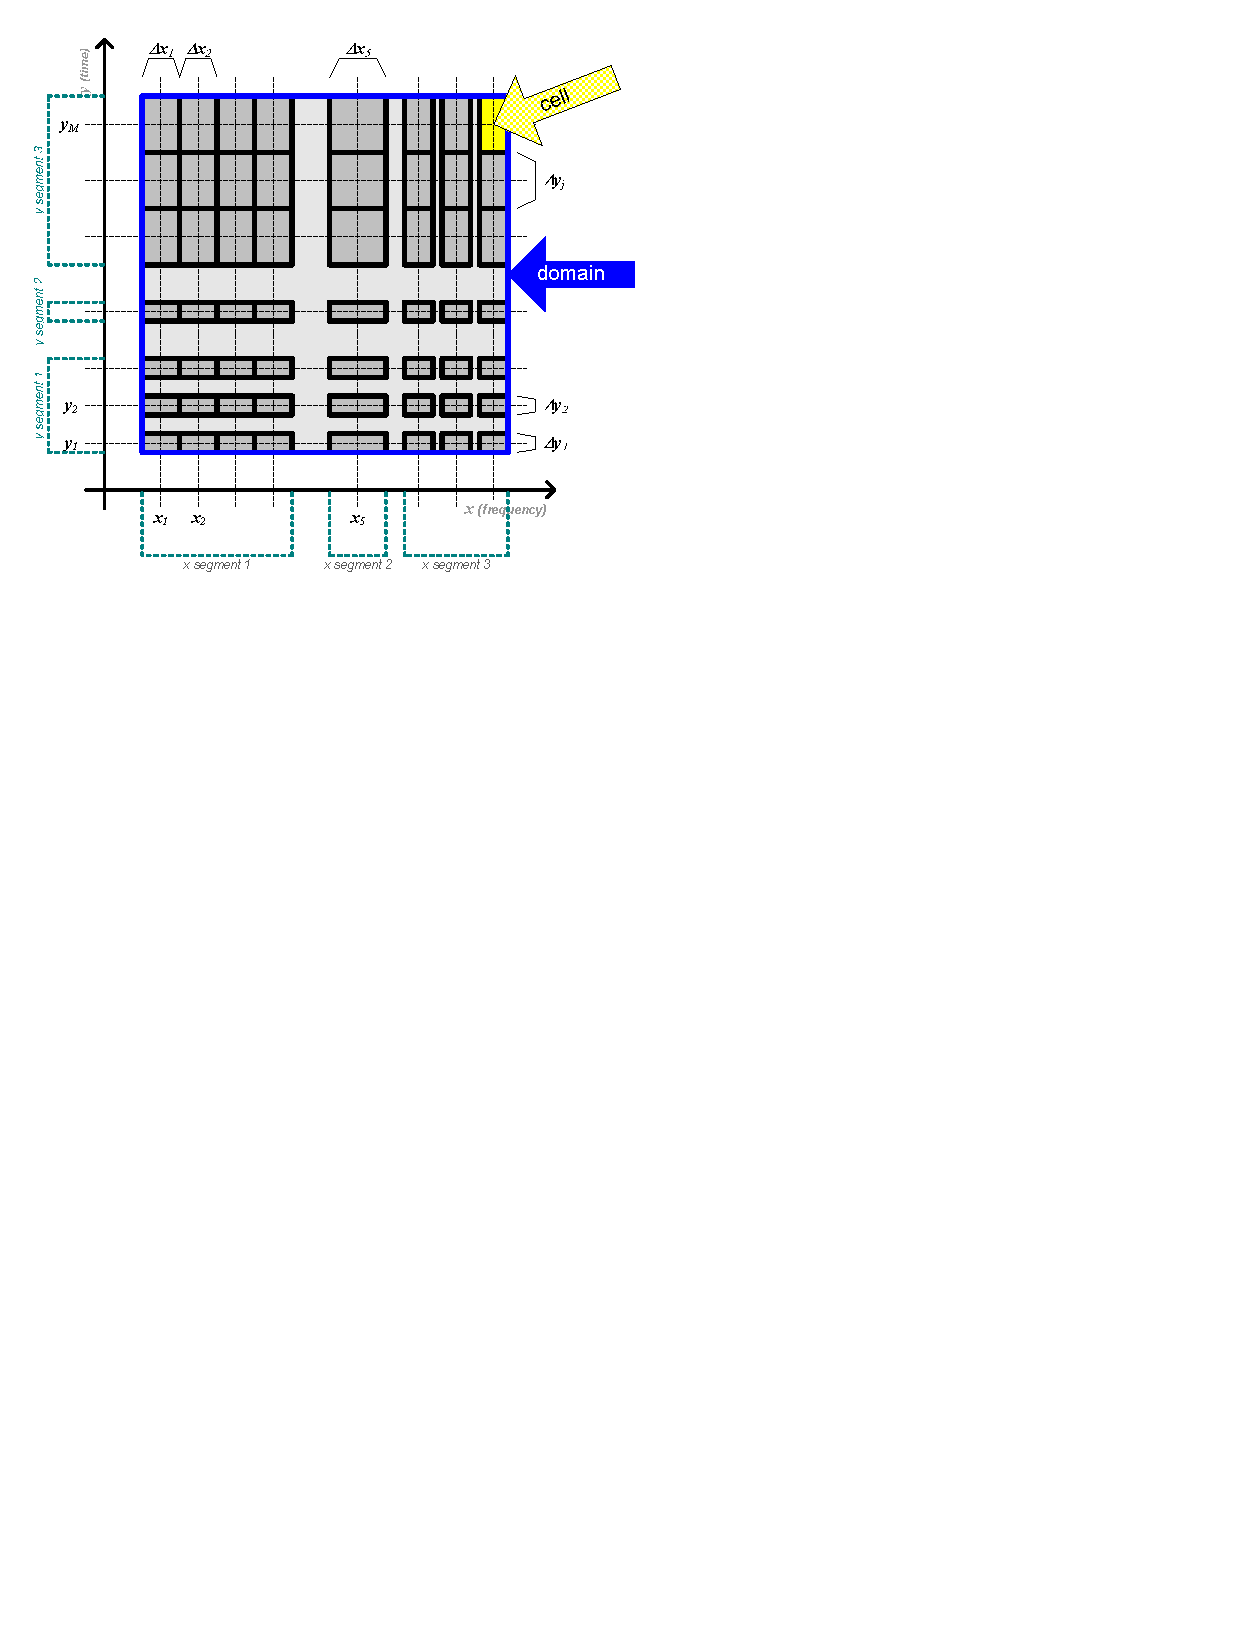
\includegraphics[width=.5\textwidth]{Figures/Cells.eps}\\
  \end{centering}
  \caption{\label{fig:cells}Layout of a Cells object and the envelope Domain}
  \end{figure}
  
  On the C++ side, both classes are derived from \qq{DataRecord}. A \Domain\ 
  record corresponding to $[f_{st},f_{end}]\times[t_{st},t_{end}]$ has the following structure:
  
  \qq{[ freq = [ $f_{st},f_{end}$ ], time = [ $t_{st},t_{end}$ ] ]}
  
  where $f_{st},f_{end},t_{st},t_{end}$ are \qq{double} values giving the domain
  boundaries.

  Note that the specific concepts of {\em frequency} and {\em time} are
  meaningful to only a handful of nodes. The majority of nodes simply deal in
  functions defined over abstract 2D space (to be precise, with 
  $\mathcal{R}^2\rightarrow\mathcal{R}$ or
  $\mathcal{R}^2\rightarrow\mathcal{C}$ functions), without associating any
  semantics with the dimensions. For this reason, the bulk of kernel code is
  careful to abstract itself from the \qq{freq} and \qq{time} names whereever
  possible, treating domain components only as ``first axis'' and ``second
  axis''. The Glish syntax of selecting record fields by number is handy here:
  if \qq{dom} is a domain record, then \qq{dom[1]} and \qq{dom[2]} refer to the
  axis subrecords in a name-independent way.

  The \Cells\ record is structured in the same spirit:
  
  {\tt\begin{tabular}{lrl@{}l}
  [ &domain~&     = [ {\em envelope domain record} ],\\
    &grid~&       = [ freq = [$f_1,...,f_N$],~&~time = [$t_1,...,t_M$] ],\\
    &cell\_size~& = [ freq = [$\Delta f_1,...,\Delta f_N$],~&~time = 
                              [$\Delta t_1,...,\Delta t_M$] ],\\
    &segments&\multicolumn{2}{l}{=~[ freq =
    [start\_index=[$i'_1,...,i'_n$],end\_index=[$i''_1,...,i''_n$]],}\\
              &&\multicolumn{2}{l}{~~~~time =
              [start\_index=[$j'_1,...,j'_m$],end\_index=[$j''_1,...,j''_m$]] ] ]}\\
  \\ 
  \end{tabular}}
  
  This represents an $N\times M$ gridding of the given domain. The $\{f_i\}$ and
  $\{t_j\}$ vectors give the cell centers, while $\{\Delta f_i\}$ and $\{\Delta
  t_j\}$ give the cell sizes. 
  
  The \qq{segments} sub-record contains information on the {\bf regular
  segments} of the grid.\footnote{Some calculations, such as the DFT, can be
  significantly optimized over regular grids.} A regular segment is a part of
  the grid over which the stepping between cell centers, as well as the cell
  size, remains constant. The \qq{start\_index} and \qq{end\_index} vectors
  contain the starting ($i',j'$) and ending ($i'',j''$)
  indices\footnote{1-based in Glish, 0-based in C++, see
  section~\ref{sec:indexconv}.} of each regular segment.
  By definition, given $n$ segments and $N$ grid points, $i'_{k}= i''_{k-1}+1$,
  $i'_1=1$, $i''_n=N.$

  In the simplest case, the entire $N\times M$ grid is regular, in which case the
  \qq{segments} subrecord looks like this:
 
  {\tt\begin{tabular}{ll}
  [&freq=[start\_index=[1],end\_index=[$N$]],\\
  &time=[start\_index=[1],end\_index=[$M$]]~~~~]\\
  \end{tabular}}
  
  The other extreme, of course, is the completely irregular grid. This is
  represented by \qq{segments} of the form:

  {\tt\begin{tabular}{ll}
  [&freq=[start\_index=[1,2,$...N$],end\_index=[1,2,$...N$]],\\
  &time=[start\_index=[1,2,$...M$],end\_index=[1,2,$...M$]]~~~~]
  \end{tabular}}
  
  Figure~\ref{fig:cells} shows an $8\times7$ grid with three regular segments
  along each axis. This would correspond to the following \qq{segments}
  sub-record:

  {\tt\begin{tabular}{ll}
  [&freq=[start\_index=[1,5,6],end\_index=[4,6,8]],\\
   &time=[start\_index=[1,4,5],end\_index=[3,5,7]] ]
  \end{tabular}}
  
  Note that \qq{segments} information is merely an optimization facility, and
  can be safely ignored most of the time. The user need not know anything about
  it, since \Cells\ constructors compute \qq{segments} automatically; most
  application code doesn't care either, instead working directly with the
  \qq{grid} vectors. 

  On a related note, the \Cells\ record is full of redundant information. For
  example, \qq{domain} and \qq{segments} can be completely derived from
  \qq{grid} and \qq{cell\_size}. This has two important implications:
  
  \begin{itemize}
  
  \item To construct a \Cells, you need to provide only the minimum sufficient
  information, while the constructor figures out everything else automatically.

  \item \Cells\ records should be treated as read-only. Directly manipulating 
  any of the values inside can break consistency between the
  grid/domain/segments fields, and lead to all sorts of confusion down
  the line.

  \end{itemize}

\subsubsection{Empty \Cells{}}

  An empty record corresponds to an uninitialized \Cells\ object in C++. Empty
  \Cells\ may appear in situations where the cell information is not defined,
  so Glish code should be prepared to deal with it. See
  section~\ref{sec:result-empty-cells} for an example.
  
  
\subsubsection{Constructing \Domain{}s and \Cells{}}

  The Glish \qq{meq.domain{}} function constructs a record corresponding to
  a \Domain\ object. Its usage is pretty much self-evident:
  
  \begin{verbatim}
    meq.domain := function (startfreq,endfreq,starttime,endtime)
  \end{verbatim}
  
  The \qq{meq.cells()} function is somewhat more elaborate:
  
  \begin{verbatim}
    const meq.cells := function (domain=F,num_freq=F,num_time=F,
                                 freq_grid=[],time_grid=[],
                                 freq_cell_size=[],time_cell_size=[])
  \end{verbatim}

  All of the arguments are optional, allowing different ways of specifying 
  a \Cells. For example,
  
  \qq{~~cells := meq.cells(meq.domain(0,1,0,1),2,2);}
  
  creates a regular $2\times 2$ grid for the domain $[0,1]\times[0,1]$: cell
  centers at (0.25,0.75), cell sizes of (0.5,0.5). The same \Cells\ can be
  alternatively specified as:
  
  \qq{~~cells := meq.cells(freq\_grid=[0.25,0.75],time\_grid=[0.25,0.75]);}
  
  letting the constructor derive the domain \& cell size automatically. The
  two forms can even be mixed:
  
  \qq{~~cells := meq.cells(meq.domain(0,0,0,1),freq\_grid=[0.25,0.75],num\_time=2);}
  
  produces the same \Cells\ yet again -- note that the \qq{freq\_grid} 
  values override the \qq{freq} component of the domain.
  
  If not supplied in the function call, the default cell sizes are computed to
  perfectly tile the specified domain. The \qq{freq\_} and
  \qq{time\_cell\_size} arguments allow you to supply explicit cell sizes.
  These may be scalars -- implying the same size for all cells along that axis
  -- or vectors. In the latter case, the size of the vector must match
  the corresponding \qq{$x$\_grid} or \qq{num\_$x$} argument.

\section{Fail-records and fail-states}
  \label{sec:fail}

  Run-time errors during execution are reported via special structures called
  fail-records. Because fail-records can appear within different data
  structures (see below), they deserve to be documented separately. A
  fail-record has the following layout: \vspace{1em}

  \noindent\begin{tabular}{l|l|p{.7\textwidth}}
  \hline
  {\scriptsize\sf field name } & {\scriptsize\sf type} & {\scriptsize\sf description}\\
  \hline
  \qq{message} & \qq{string} & a description of the error.\\
  \qq{node\_name} & \qq{string} & {\em [optional]}~~name of originating node, if any.\\
  \qq{node\_class} & \qq{string} & {\em [optional]}~~classname of originating node, if any.\\
  \qq{origin} & \qq{string} & origin: usually just the source file name.\\
  \qq{origin\_line} & \qq{int} & origin location: usually just the source line number.\\
  \hline
  \end{tabular}\vspace{1em}
  
  Because most errors tend to cascade from lower-level subsystems up to the
  application level, accumulating more specific descriptions along the way,
  fail-records usually come in a list. Lower-level errors then appear up at the
  head of the list, and higher-level errors appear at the tail.
  
  Certain data classes described below (e.g., \qq{Result} and \qq{VellSet})
  support a fail-state -- i.e., a form of the data object describing a failure.
  A fail-state is represented by a record with a single field named \qq{fail},
  containing a list of fail-records. The kernel uses this field exclusively for
  indicating fail state, so all Glish code can follow a simple policy and
  process fails in the same consistent way everywhere: 

  \begin{itemize} 
  
  \item Any record with a \qq{fail} field represents an object  in fail-state.

  \item In fail-state, no other meaningful fields exist.
  
  \item The \qq{fail} fields always contains a {\em list} of fail records (even
  if the list contains only one element).
  
  \end{itemize}
  

\section{MeqResult and related data objects}
\label{sec:Result}

  A \Result\ contains the result of a \Request's execution. A \Result\ is also
  a record (derived from \qq{DataRecord} on the C++ side). Theoretically, this
  record is completely free-form, with its contents dependant on the commands
  in the original \Request\ (and in some cases even on node type -- e.g., a
  \qq{Solver}'s result will contain solution metrics). If, however, the
  original \Request\ contains a \qq{cells} command -- asking the node to
  evaluate itself over the given \Cells\ -- and the command is executed
  successfully, then the returned \Result\ has a well-defined structure:
  \vspace{1em}

  \noindent\begin{tabular}{l|l|p{.7\textwidth}}
  \hline
  {\scriptsize\sf field name } & {\scriptsize\sf type} & {\scriptsize\sf description}\\
  \hline
  \qq{cells}  & \Cells & the \Cells\ of the result (not necessarily matching the request cells
  -- see discussion below)\\
  \qq{values} & \qq{VellSet[]} & list of result values\\
  \qq{integrated} & \qq{bool} & flag indicating if the values are integrations or
                    samplings (default is false, implying samplings)\\
  \hline
  \end{tabular}\vspace{1em}
  
  Two other common types of \Result\ are the empty result (empty record),
  returned when a \Request\ does not contain any commands with return values,
  and the fail-result (see section~\ref{sec:fail}), returned when a run-time
  error arises during execution. 
    
\subsection{Sampling vs. integration}
  \label{sec:integration}
  
  A \Result\ can represent both a sampling of some function at the cell
  centers, or an integration over each cell. The \qq{integrated} flag is used
  to indicate this, if missing, \qq{false} (i.e. a sampling) is assumed. Leaf
  nodes set this flag according to the type of value they return (for example,
  a \qq{Spigot} reading visibilities from a data set returns integrations; a
  \qq{Parm} representing gain returns samplings). Non-leaf nodes should take
  care to pass this flag from child to parent properly. This flag is also taken
  into account when performing resampling of results
  (section~\ref{sec:resampling}).

\subsection{Multiple values}
  
  Note that the \qq{values} field is defined as a {\em list} of \VellSet{}s. In
  Glish, a list is implemented as a record, using the \qq{rec[1]}, \qq{rec[2]},
  etc. syntax to access fields by number. Even if there is only one \VellSet\
  in the list, you still have to access it as \qq{result.values[1]}.

  Each \VellSet\ represents a function $f:\RR^2\rightarrow\RR$ or $\CC$. A set
  of $N$ \VellSet{}s then represents $f:\RR^2\rightarrow\RR^{N}$ or
  $\CC^{N}$.\footnote{In fact, the set can even contain a mix of $\RR$ and
  $\CC$ codomains.} Another way to look at it is that a set of \VellSet{}s
  allows multiple ``planes'' for a single \Cells. For example, a \qq{Spigot}
  may return four planes at a time for the four correlations. Function nodes
  expect all child \Result{}s to either have the same number of planes, and
  will apply the function to each set of planes (cross-slice) independently;
  however, some children may have only one plane, in which case it is re-used
  in each cross-slice.

  The \qq{Selector} and \qq{Composer} nodes can be used to decompose and
  assemble \Result{}s on a plane-by-plane basis. The \qq{Selector} node has one
  child; it returns a \Result\ composed of specific plane(s) from its child. The
  \qq{Composer} assembles a \Result\ from all the planes returned by its
  children.

\subsection{VellSet}

  A \VellSet\ is essentially a sampling or integration
  (see~\ref{sec:integration}) of some function
  $f:\mathcal{R}^2\rightarrow\mathcal{R}$ or 
  $f:\mathcal{R}^2\rightarrow\mathcal{C}$ over a certain \Cells. A \Cells\ 
  defines a domain \& grid in $\mathcal{R}^2$ space -- usually interpreted as
  frequency-time -- specified by the grid vectors $(x_1,...,x_N)$ and
  $(y_1,...,y_M)$. Thus, a \VellSet\ contains an $N\times M$ matrix of {\em
  function values} $f_{ij}=f(x_i,y_j)$.

  If the function is dependent on $K$ real parameters $(p_1,...,p_K)$, then the
  \VellSet\ may also contain a set of {\em perturbed values}
  $\{f^{(k)}_{ij}\}$, which can be used to estimate the partial derivatives
  $\partial f/\partial p_k$. The math behind this is explained in
  section~\ref{sec:math}. Within a tree, the parameters $p_k$ are uniquely
  indentified by their integer {\bf spids} (from {\em solvable parameter IDs}\/).

  On the C++ side, \VellSet\ is derived from \qq{DataRecord}. The \VellSet\
  record has three forms: regular, empty and fail.
  
\subsubsection{Regular VellSets}
  
  The regular form of a VellSet contains the following fields:

  \vspace{1em}
  
  \noindent\begin{tabular}{l|l|p{.7\textwidth}}
  \hline
  \qq{value}  & \qq{Vells} & the \Vells\ containing the function value $\{f_{ij}\}$\\\hline
  \multicolumn{3}{l}{~~~~\em optional, only appear if \qq{calc\_deriv>0} was specified in
  the original \Request:}\\
  
  \qq{spids}  & \qq{int[]} & a list of $K$ integer spids identifying the parameters\\
                
  \qq{perturbations} & \qq{double[]} & a list of $K$ perturbations $\{\delta_k\}$ (must be same length as \qq{spids})\\
  
  \qq{perturbed\_value} & \qq{Vells[]} & a list of $K$ \Vells\ containing the perturbed values
                      $\{f^{(k)}_{ij}\}$\\\hline

  \multicolumn{3}{l}{~~~~\em optional, only appear if \qq{calc\_deriv>1} was specified 
  in the original \Request:}\\
  
  \qq{perturbations\_1}  & \qq{double[]} & second set of $K$ perturbations
  $\{\delta^\prime_{k}\}$\\

  \qq{perturbed\_value\_1} & \qq{Vells[]} & second set of $K$ perturbed values
  $\{f^{(k)\prime}_{ij}\}$\\
  \hline
  
  \end{tabular}\vspace{1em}

  Spids, perturbations and perturbed values will only appear if
  \qq{calc\_deriv} is specified in the original \Request, and the tree above
  the node contains solvable parameters. A setting of \qq{calc\_deriv=2} causes
  two sets of perturbations and perturbed values to be computed (usually
  $\delta^\prime_k=-\delta_k$), used to estimate the second-order
  derivatives of $f$, which (usually) facilitates a better fit, while doubling
  computing time.

  \subsubsection{Empty VellSets}

  An empty \VellSet\ is just an empty record, corresponding to a
  default-constructed (empty) object in C++. While empty \VellSet{}s shouldn't
  be present in well-formed results, they can still appear in node state
  records and other structures, thus Glish code should be prepared to deal with
  them.
  
  \subsubsection{Fail-VellSets}

  A fail-VellSet is used to indicate a run-time error or other failure. This
  is represented by a standard fail-state record (see section~\ref{sec:fail}).
  The difference between this and a fail-Result is discussed below.

\subsubsection{Vells}

  On the Glish side, a \Vells\ object is simply a \qq{double} or \qq{complex}
  scalar or a 2D array. On the C++ side, \Vells\ is a wrapper class around the
  scalar/array, providing some run-time type and size information, and built-in
  mathematical operations (see \qq{Function} nodes, section~\ref{sec:Function}).

  Scalar \Vells\ represent values with no time-frequency variation. Array
  \Vells\ represent dependence {\em over a specific Cells.} This implies that
  all array \Vells\ within a valid \Result\ must be consistent (in shape) with
  the \Result's \Cells.

\subsection{Empty Cells in Results}
  \label{sec:result-empty-cells} 
  
  A \Result\ record containing an empty \Cells\ field is used to represent {\em
  constant values} -- or values with no time-frequency dependence. In other
  words, a \Result\ with an empty \Cells\ will remain the same for any possible
  set of real cells. Such a \Result\ may only contain scalar \Vells. This
  property of a \Result\ is important during resampling
  (see~{\ref{sec:resampling}), since constant values do not need to be
  resampled.

\subsection{Fail propagation}

  Note that a \Result\ that is not in a fail-state itself may nonetheless
  contain one or more \VellSet{}s in a fail-state. One way to look at it is that a 
  fail-Result represents a complete fail, while a fail-VellSet represents a
  partial fail localized to one plane. For example, if a \qq{Spigot} node is
  configured to return four correlations, and the data source only contains
  $XX$ and $YY$, then the $XY$ and $YX$ planes will be represented by
  fail-VellSets. On the other hand, if an error occurs while reading from the
  data set, this is represented by a complete fail-Result.

  Depending on the tree, partial fails may be recoverable. Fails propagate down
  the tree in an orderly fashion. For most nodes, a partial fail from one of
  its children will result in a fail-VellSet at the same position in the output
  \Result\ (the contents of the fail -- origin \& description -- are
  preserved.) In our example, partial fails could propagate down the $XY$/$YX$
  trees, to a \qq{Sink} node, which could then handle them benignly (by not
  writing XY/YX data, for example). Partial fails can even ``disappear'' on
  their way down a tree -- consider a \qq{Selector} node that is configured
  to select plane 1 of the \Result. Partial fails in the other planes will
  simply be discarded.


